%======================================================================
Per poter gestire e programmare la movimentazione del manipolatore ABB IRB 120 è necessario effettuare uno studio della sua cinematica (figura~\vref{fig:Cinematica_DirInv}), ovvero di quello che è il legame tra lo stato dei 6 giunti e la posizione e l'orientamento dell'end-effector: questo legame deve essere gestito in base a quelli che sono i sistemi di riferimento principali e le dimensioni geometriche riguardanti il manipolatore.

Analizzeremo innanzitutto quelli che sono i sistemi di coordinate utilizzati per definire la movimentazione del manipolatore ABB IRB 120, andando poi a sviluppare uno studio della cinematica diretta e inversa del manipolatore stesso, fornendo così gli strumenti necessari, a livello matematico, per definire con precisione le coordinate spaziali del robot.

\begin{figure}[h]
	\centering
	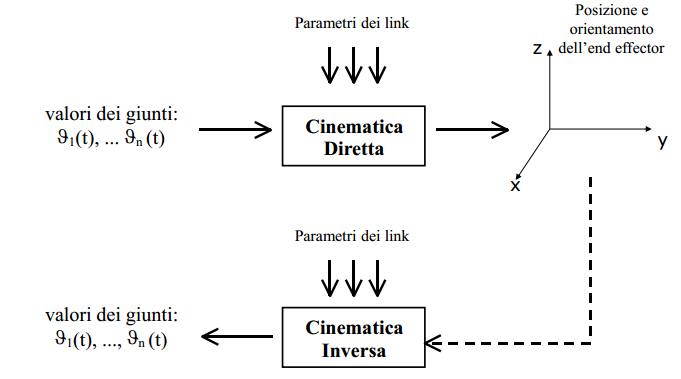
\includegraphics[width=0.7\textwidth]{Immagini/Cinematica_inv_dir_scheme}
	\caption{Cinematica diretta e inversa\cite{rep:Slide_Brugali1}}
	\label{fig:Cinematica_DirInv}
\end{figure}



\subsection{Sistemi di coordinate}

Come già ribadito in precedenza, quello che si vuole andare a gestire è la traiettoria del manipolatore, ovvero la posizione dell'end effector: questo però è possibile solo dal momento in cui si definisce un punto di riferimento rispetto al quale si riferisce il moto, ovvero definendo un origine dalla quale si sviluppa poi un sistema di coordinate bi o tridimensionale. 

Nell'ambiente di sviluppo RobotStudio (capitolo~\vref{text:RobotStudio}) si lavora con più sistemi di riferimento, permettendo la creazione di aree di lavoro complesse; questi specifici sistemi di coordinate, che permettono una gestione del moto nell'area di lavoro più articolata, semplificando nello stesso tempo la programmazione fuori linea, sono:
\begin{figure}[h]
	\centering
	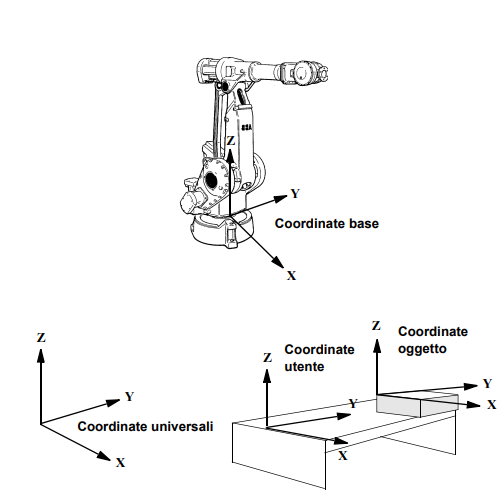
\includegraphics[width=0.7\textwidth]{Immagini/SistemiDiCoordinate}
	\caption{Sistemi di riferimento esterni per la gestione della traiettoria del manipolatore}
	\label{fig:SdR}
\end{figure}
\begin{description}
	\item[Sistema di coordinate universale:] definito anche WCS \emph{(World Coordinate System)}, definisce un riferimento rispetto al pavimento o alla cella di lavoro, che rappresenta il punto di partenza per gli altri sistemi di coordinate. Utilizzando questo sistema di coordinate, è possibile mettere in relazione la posizione del robot con un	punto fisso in fabbrica, per esempio. 
	Risulta quindi essere molto utile quando due robot lavorano insieme, dovendo collaborare tra di loro.
	
	\item[Sistema di coordinate della base:] esso ha come origine il punto centrale alla base del robot, ovvero la base d'appoggio del robot.
	
	\item[Sistema di coordinate dell'utente:] esso specifica la posizione di un'attrezzatura esterna, fornendo così la possibilità di inserire sistemi di	coordinate 	per diversi attrezzi e/o superfici di lavoro. 
	
	\item[Sistema di coordinate dell'oggetto di lavoro:] in sistemi di lavoro, anche di media complessità, un attrezzo potrebbe includere vari oggetti di lavoro che devono essere elaborati o gestiti dal robot.	
	Questo	consente di definire un sistema di coordinate per ogni oggetto (si possono quindi avere più sistemi di coordinate di questo tipo) per poter regolare
	più facilmente il programma nel caso in cui un oggetto venga spostato oppure un
	nuovo elemento, simile a quello precedente, debba essere programmato in una diversa posizione, permettendo una ridefinizione automatica della traiettoria. 
	
	Esso viene ad essere posizionato rispetto al sistema di coordinate utente, riuscendo ad adattarsi perfettamente alla programmazione off-line, in quanto le posizioni specificate	possono essere ricavate direttamente da un disegno del work object, ovvero dell'area di lavoro (detta alternativamente anche workstation).
	\item[Sistema di coordinate del polso:]\label{item:SdR_Polso} esso rappresenta il sistema di riferimento del giunto numero 6; in sostanza, come per gli altri 5 assi, esso permette di definire la posizione del centro del giunto stesso. Merita una menzione particolare poichè questo sistema di riferimento definisce l'orientamento del manipolatore (figura~\vref{fig:axis6}).
	\begin{figure}[h]
		\centering
		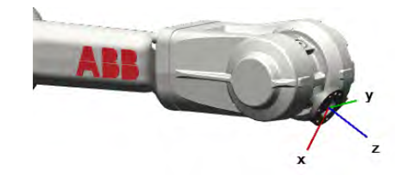
\includegraphics[width=0.5\textwidth]{Immagini/SistemaDiRiferimento_Polso}
		\caption{Sistema di coordinate polso}
		\label{fig:axis6}
	\end{figure}
	\item[Sistema di coordinate dell'utensile di lavoro:]\label{item:TCP} esso permette di definire la posizione e l'orientamento dell'utensile agganciato al polso. Spesso chiamato TCP \emph{(Tool Center Point)} la sua importanza è quindi estrema, poichè permette di gestire il punto con il quale il manipolatore andrà ad agire direttamente sull'oggetto, definendone la gestione della lavorazione/manipolazione richiesta (figura~\vref{fig:TCP})
\end{description}
\begin{figure}[h]
	\centering
	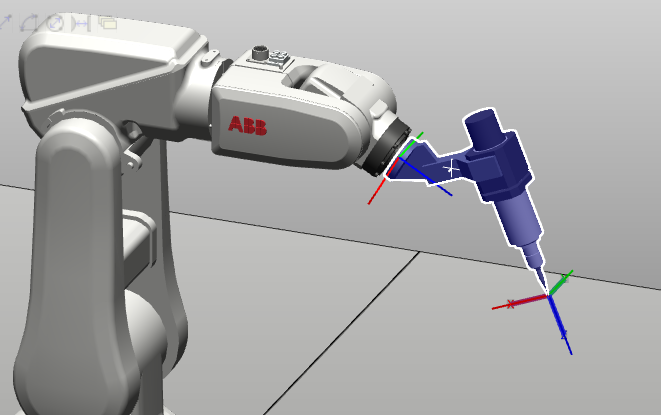
\includegraphics[width=0.5\textwidth]{Immagini/TCP}
	\caption{Tool Center Point}
	\label{fig:TCP}
\end{figure}
Da queste brevi descrizioni si capisce come la gestione della traiettoria del manipolatore debba occuparsi della posizione e dell'orientamento del \emph{TCP} rispetto al sistema di riferimento oggetto: entrambi risultano essere definiti, a loro volta, rispetto al sistema di coordinate universale.



\subsection{Descrizione di posizione e orientamento di un sistema di riferimento}
Come si può vedere in figura~\vref{fig:Catena_Cinematica}, l'ABB IRB 120 può essere modellizzato come un insieme di sistemi di riferimento: trattandosi infatti di un manipolatore robotico, esso è costituito da una sequenza di organi meccanici \emph{(links)}, collegati tra loro da \emph{joints}, i quali permettono di individuare così una catena cinematica aperta, per l'assenza di anelli chiusi.
\begin{figure}[h]
	\centering
	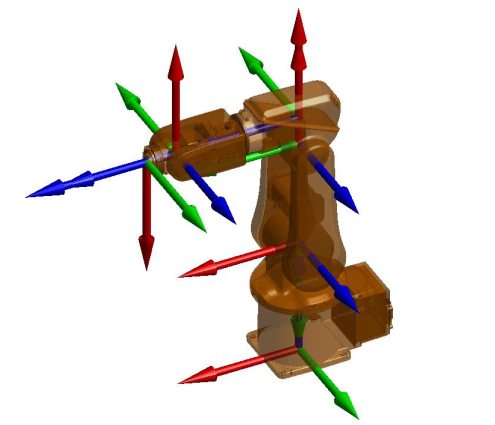
\includegraphics[width=0.6\textwidth]{Immagini/CatenaCinematica}
	\caption{Catena cinematica IRB 120}
	\label{fig:Catena_Cinematica}
\end{figure}

Ad ogni link è associato un sistema di coordinate che ne caratterizza la posizione: quindi il fulcro del problema cinematico si riduce alla definizione della posizione e dell'orientamento di un generico sistema di riferimento, sfruttando poi le caratteristiche della catena cinematica (figura~\vref{fig:Catena_Cinematica}) per andare a posizionare il robot.

La posizione di un sistema di riferimento è banalmente individuata dalle coordinate $x,y,z$ della sua origine, sempre riferite ad un sistema fissato: ciò che comporta uno studio più approfondito è l'orientamento di una terna rispetto ad un'altra, possibile andando ad utilizzare i versori della prima terna rispetto a quelli della seconda (figura~\vref{fig:Rotazione_SistemaDiRiferimento}).
\newpage
\subsubsection{Rotazioni elementari}
\label{subsub:Rot_elementari}
\begin{figure}[h]
	\centering
	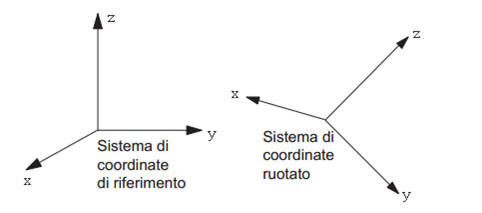
\includegraphics[width=0.6\textwidth]{Immagini/Rotazione_SistemiDiRiferimento}
	\caption{Rotazione di una terna rispetto ad un'altra}
	\label{fig:Rotazione_SistemaDiRiferimento}
\end{figure}
 Riferendosi alla figura~\vref{fig:Rotazione_SistemaDiRiferimento}, andando a far coincidere le origini delle due terne, ovvero operando una traslazione della seconda terna rispetto alle prima, possiamo vedere i versori dei tre assi traslati come tre vettori separati, i quali possono quindi essere espressi rispettivamente come:
 \begin{itemize}
 	\item $\hat{\vec{x}}= $ versore dell'asse $ x=(x_1,x_2,x_3)\Rightarrow$ Il versore direzionale dell'asse x  presenta una componente $x_1$ lungo l'asse x del sistema di riferimento considerabile \emph{fisso}, $x_2$ lungo y e $x_3$ lungo z.
 	\item $\hat{\vec{y}}=$ versore dell'asse $y=(y_1,y_2,y_3)\Rightarrow$ Il versore direzionale dell'asse y  presenta una componente $y_1$ lungo l'asse x del sistema di riferimento considerabile \emph{fisso}, $y_2$ lungo y e $y_3$ lungo z.
 	\item $\hat{\vec{z}}=$versore dell'asse z$=(z_1,z_2,z_3)\Rightarrow$ Il versore direzionale dell'asse z  presenta una componente $z_1$ lungo l'asse x del sistema di riferimento considerabile \emph{fisso}, $z_2$ lungo y e $z_3$ lungo z.
 \end{itemize}
La matrice di rotazione prende quindi la seguente forma: il pedice posto alla sinistra dellla matrice indica il sistema di riferimento descritto, mentre l'apice indica il riferimento usato per la descrizione, ovvero la matrice \textbf{R} (matrice~\vref{mat:RotationMatrix}) indica la matrice di rotazione che descrive la terna $\{$B$\}$ rispetto alla terna $\{$A$\}$.
\begin{equation}
	\label{mat:RotationMatrix}	
	\textbf{$\prescript{A}{B}{\textsc{R}}$}=
	\begin{bmatrix}
	x_1&y_1&z_1\\
	x_2&y_2&z_2\\	
	x_3&y_3&z_3
	\end{bmatrix}
	=
	\begin{bmatrix}
	\hat{\vec{x_B}}\cdot\hat{\vec{x_A}}&\hat{\vec{y_B}}\cdot\hat{\vec{x_A}}&\hat{\vec{z_B}}\cdot\hat{\vec{x_A}}\\
	\hat{\vec{x_B}}\cdot\hat{\vec{y_A}}&\hat{\vec{y_B}}\cdot\hat{\vec{y_A}}&\hat{\vec{z_B}}\cdot\hat{\vec{y_A}}\\	
	\hat{\vec{x_B}}\cdot\hat{\vec{z_A}}&\hat{\vec{y_B}}\cdot\hat{\vec{z_A}}&\hat{\vec{z_B}}\cdot\hat{\vec{z_A}}
	\end{bmatrix}
\end{equation}
La matrice~\vref{mat:RotationMatrix} è detta anche matrice dei coseni direttori dato che, per definizione di prodotto vettoriale ($\hat{\vec{x_B}}\cdot\hat{\vec{x_A}}=\parallel\hat{\vec{x_B}}\parallel\cdot\parallel\hat{\vec{x_A}}\parallel\cdot\cos \alpha=\cos\alpha$), i componenti della matrice di rotazione saranno solamente dei coseni degli angoli compresi tra i versori.
\begin{figure}
	\centering
	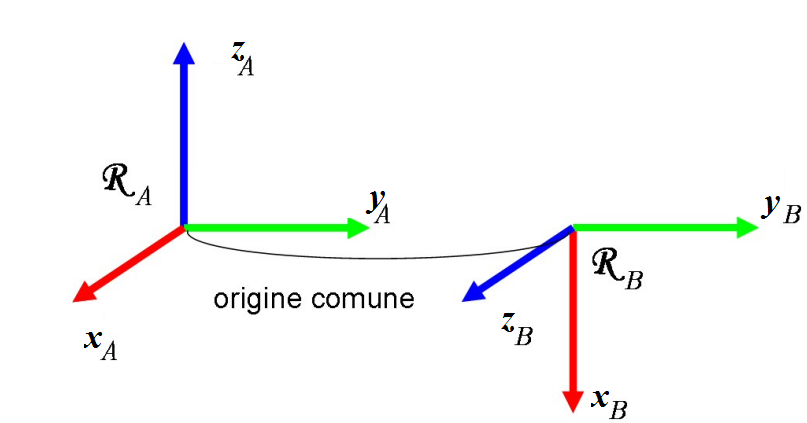
\includegraphics[width=0.5\textwidth]{Immagini/EsempioRotazione}
	\caption{Semplice esempio di rotazione di sistemi di riferimento}
	\label{fig:ShortExampleRotationMatrix}
\end{figure}
\newpage
Per poter trovare la semplice matrice di rotazione che descrive la rotazione in figura~\vref{fig:ShortExampleRotationMatrix}, le due possibilità che si hanno sono quelle di
\begin{itemize}
	\item  individuare i versori del sistema di riferimento B rispetto al sistema A.
	\item sviluppare i prodotti vettori (ricordando che esso si annulla per vettori ortogonali tra di loro).
\end{itemize} 
Detto ciò possiamo trovare la matrice come:
\begin{equation}
	\vec{x_B}=
	\begin{bmatrix}
		0\\	
		0\\
		-1
	\end{bmatrix}
	,
	\vec{y_B}=
	\begin{bmatrix}
		0\\	
		1\\
		0
	\end{bmatrix}
	,
	\vec{z_B}=
	\begin{bmatrix}
		1\\	
		0\\
		0
	\end{bmatrix}
\end{equation}
La matrice di rotazione della figura~\vref{fig:ShortExampleRotationMatrix} sarà quindi:
\begin{equation}
	\label{mat:ExampleRotationMatrix}	
	\textbf{$\prescript{A}{B}{\textsc{R}}$}=
	\begin{bmatrix}
	0&0&0\\
	0&1&0\\	
	-1&0&1
	\end{bmatrix}
\end{equation}
Quelle considerate finora, tramite semplici esempi, rappresentano rotazioni elementari (figura~\vref{fig:RotazioniElementari}), ovvero che avvengono lungo un determinato asse.
Andando ad applicare quanto di semplice fatto nell'esempio in figura~\vref{fig:ShortExampleRotationMatrix}, siamo in grado di andare a trovare le matrici di rotazione per i casi di rotazioni generiche:
\begin{description}
	\item[$\bullet$ Rotazione intorno asse x di angolo $\gamma$: ] \begin{equation}
		\label{mat:RotationMatrix_x}	
		\textbf{$\textsc{R}_X(\gamma)$}=
		\begin{bmatrix}
			1&0&0\\
			0&\cos \gamma&-\sin \gamma\\
			0&\sin \gamma&\cos \gamma
		\end{bmatrix}
	\end{equation}
	\item[$\bullet$ Rotazione intorno asse y di angolo $\beta$: ] \begin{equation}
		\label{mat:RotationMatrix_y}	
		\textbf{$\textsc{R}_y(\beta)$}=
		\begin{bmatrix}
			\cos \beta&0&\sin \beta\\
			0&1&0\\
			-\sin \beta&0&\cos \beta
		\end{bmatrix}
	\end{equation}
	\item[$\bullet$ Rotazione intorno asse z di angolo $\alpha$: ] \begin{equation}
		\label{mat:RotationMatrix_z}	
		\textbf{$\textsc{R}_z(\alpha)$}=
		\begin{bmatrix}
			\cos \alpha&-\sin \alpha&0\\
			\sin \alpha&\cos \alpha&0\\	
			0&0&1
		\end{bmatrix}
	\end{equation} 
\end{description}
\begin{figure}
	\centering
	\subfloat[][Rotazione intorno a x]{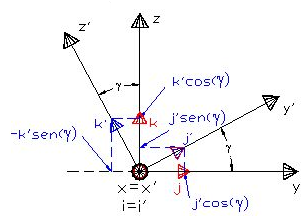
\includegraphics[width=0.40\textwidth]{Immagini/Rot_asse_x}}
	\subfloat[][Rotazione intorno a y]{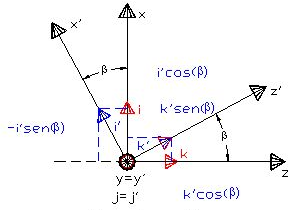
\includegraphics[width=0.40\textwidth]{Immagini/Rot_asse_y}}\\
	\subfloat[][Rotazione intorno a z]{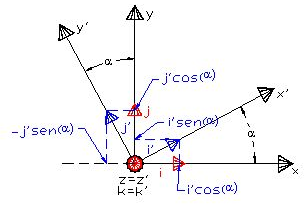
\includegraphics[width=0.40\textwidth]{Immagini/Rot_asse_z}}	
	\caption{Rotazioni elementari}
	%[Immagine presa dal sito http://slideplayer.it/slide/537558/ in data 03/03/18] 
	\label{fig:RotazioniElementari}
\end{figure}

\subsubsection{Composizione delle matrici di rotazione: rotazioni complesse}
\label{subsubsection:RotComplex}
Concetto importante, che poi riapparirà, seppur se in forma più complessa, nella convenzione di Denavit-Hartenberg (sottosezione~\vref{subsubsection:D-H}), è quello di \emph{composizione delle matrici di rotazione}.

Finora sono state analizzate solamente rotazioni di tipo elementare, ovvero che avvengo intorno ad un unico asse: ogni altra rotazione, e la corrispondente matrice, possono essere ottenuti combinando opportunamente le rotazioni elementari.

\label{text:ComposizioneRotazioni}Si tratta quindi di scomporre la rotazione complessiva in tante rotazioni elementari: la matrice complessa è sempre ottenibile dal prodotto delle matrici di rotazioni associate alle singole sotto rotazioni "sequenziali" che possono essere effettuate in 
\begin{itemize}
	\item Terna fissa: la rotazione avviene sempre intorno agli assi del sistema di riferimento "iniziale", che viene mantenuto fisso e costante durante tutte le rotazioni sequenziali.
	\item Terna mobile: in questo caso la rotazione viene eseguita rispetto al sistema di coordinate ottenuto dalla precedente rotazione.
\end{itemize}
\begin{figure}
	\centering
	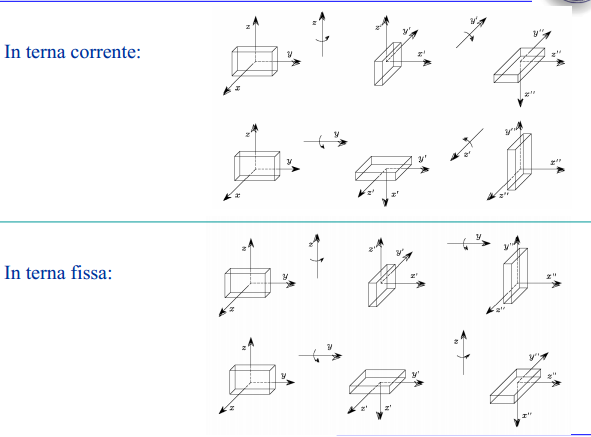
\includegraphics[width=0.75\textwidth]{Immagini/Rot_TernaFissaMobile}
	\caption{Composizione di rotazioni in terna fissa e mobile \cite{book:RobotIndustriali}}
	\label{fig:Rot_TernaFissa_Mobile}
\end{figure}
Il concetto importante è però che, indipendentemente dal tipo di rotazione composta che si va a considerare (se rispetto ad una terna fissa oppure mobile), per poter descrivere rotazioni complesse è sufficiente effettuare una moltiplicazione matriciale tra le matrici di rotazione di ogni singolo orientamento elementare.

Per esempio, supponendo di avere tre terne A, B e C diversamente orientate, si può individuare la matrice di rotazione che esprime l'orientamento della terna C rispetto ad A ($\prescript{A}{C}{\textsc{R}}$) con una moltiplicazione matriciale di questo tipo
\begin{equation}
	\prescript{A}{C}{\textsc{R}}=\prescript{A}{B}{\textsc{R}} \prescript{B}{C}{\textsc{R}}
\end{equation}
Va da se che, unendo le informazioni in merito a posizione e rotazione di un sistema di riferimento, si è in grado di individuare in maniera univoca una terna mobile rispetto ad una fissa. 

Tipicamente tale descrizione reciproca tra terne è espressa mediante una singola matrice che comprende sia le informazioni di posizione che di orientamento, la quale prende il nome di \emph{matrice di trasformazione omogenea} ed è così definita
\begin{equation*}
	\label{equation:MatrixOmogenous}
	\left[
	\begin{array}{l|r}
		\prescript{A}{B}{\textsc{R}}&pos\ped{B,A}\\ \hline
		\vec{0} & \vec{1}
	\end{array}
	\right]
\end{equation*}



\newpage
\subsection{Cinematica diretta IRB 120}

Il problema cinematico diretto si impone a di trovare il posizionamento dell'end-effector dato il valore dei giunti del manipolatore: nello specifico l'IRB 120 fa parte della categoria dei bracci seriali, ovvero di quei manipolatori costituiti da una catena cinematica aperta, composti da una sola sequenza di \emph{link} che connette i due estremi del robot stesso.
\begin{figure}[h]
	\centering
	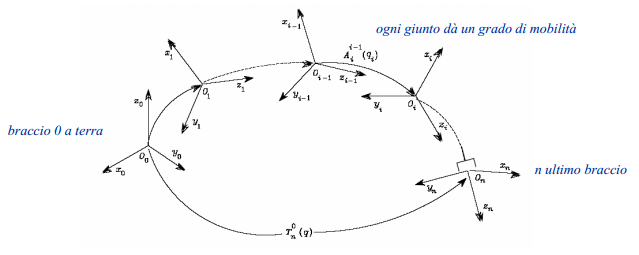
\includegraphics[width=0.75\textwidth]{Immagini/CatenaCinematicaOpen_Example}
	\caption{Esempio di catena cinematica aperta formata da \emph{n} bracci \cite{book:RobotIndustriali}} 
	\label{fig:CatenaCinematicaOpen}
\end{figure}
La risoluzione della cinematica diretta dell'IRB 120 è concettualmente molto semplice: si tratta di applicare una composizione di rotazioni in terna fissa a sistemi di riferimento solidali ad ognuno dei 6 bracci, partendo dalla terna base, ed ottenendo così orientamento e posizione dall'ultima terna della catena (end-effector) espressa rispetto alla base del manipolatore.

La composizione di rotazioni analizzata nella sottosezione~\vref{text:ComposizioneRotazioni} era riferita alle sole matrici di rotazioni, le quali individuano esclusivamente informazioni in merito all'orientamento. Questo concetto, basato su moltiplicazioni matriciali, è però applicabile anche alle matrici di trasformazione omogenea, la cui forma è leggermente più complessa (data la presenza delle informazioni in merito alla posizioni come si vede nel paragrafo~\vref{equation:MatrixOmogenous}).

Il procedimento è quindi si molto semplice: ma esiste una qualche convenzione per fissare le terne solidali ad ogni giunto (sezione ~\vref{text:joints}) in modo sistematico per facilitare la risoluzione dei prodotti matriciali?

\subsubsection{Metodo di Denavit-Hartenberg}\label{subsubsection:D-H}
Un possibile modo per poter trovare le 6 terne solidali ad ognuno degli altrettanti 6 giunti è quello di andare a posizionarle secondo il metodo di Denavit-Hartenberg: in questa sede non entreremo nei dettagli di quello che è l'algoritmo iterativo per individuare e definire la terna solidale ad ognuno dei giunti rispetto al precedente, ma ci limiteremo a rappresentarne gli aspetti più importanti e le conseguenze principali.
\newpage
La scelta dei sistemi di riferimento solidali per ogni giunto è basata quindi su due "algoritmi" iterativi:
\begin{itemize}
	\item \emph{Numerazione dei bracci e dei giunti:} ogni braccio (\emph{link}) viene numerato da 0 a \emph{n} a partire dalla base e arrivando all'organo terminale; ognuno di essi sarà individuato dai simboli $L_0,L_1,\dots,L_n$. Un manipolatore seriale, come l'IRB 120 (significa che è rappresentabile tramite una \emph{catena cinematica aperta}) con \emph{n} bracci, avrà $n-1$ giunti, designati $J_1,J_2,\dots,J_n$, dove il giunto $J_i$ collega i bracci $L\ped{i-1}$ e $L_i$.
	\item \emph{Assegnazione degli assi z dei sistemi di riferimento:} al membro \emph{i-}esimo ($0\le\emph{i}\le\emph{n}$) si associa un sistema di riferimento solidale $\{O^i,x^i,y^i,z^i\}$ il cui asse $z^i$ coincide con l'asse del giunto $J\ped{i+1}$, cioè con il giunto a valle. Come si osserva nella figura~\vref{fig:AssiZ_DH}, gli assi z dei bracci $i-1$ e $i$ hanno la stessa direzione degli assi z rispettivamente dei giunti $i$ e $i+1$.
\end{itemize}

\begin{figure}
	\centering
	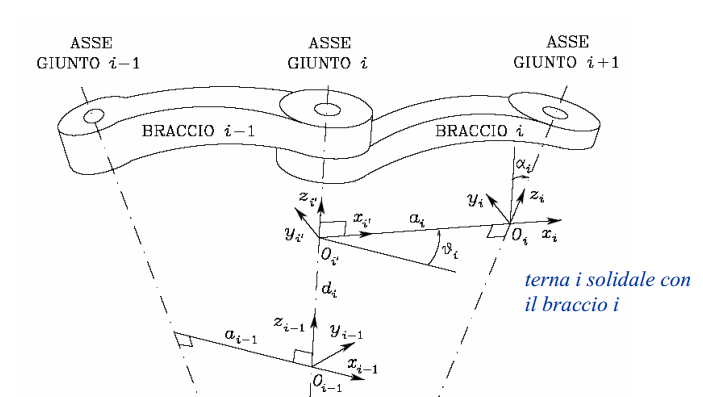
\includegraphics[width=0.75\textwidth]{Immagini/AsseZ_DH}
	\caption{Posizionamento sistemi di riferimento solidale per due bracci qualisiasi} 
	\label{fig:AssiZ_DH}
\end{figure}
Una volta assegnati gli assi $z_i$, possiamo andare a individuare:
\begin{itemize}
	\item \textsc{$O_i$}: l'origine del sistema di riferimento $i$-esimo è all'intersezione dell'asse $z_i$ con la normale comune. 
	(definibile come il segmento ortogonale agli assi del giunto $i$-esimo e di quello $i+1$-esimo, come si può vedere nella figura ~\vref{fig:AssiZ_DH}); si indica con $O^{'}_{i}$ l'intersezione della normale comune con $z\ped{i-1}$.
	\item \textsc{$x_i$}: è diretto lungo la normale comune agli assi $z_i$ e $z\ped{i-1}$, con verso positivo dal giunto $i$ al giunto $i+1$
	\item \textsc{$y_i$}: completa la terna destrorsa.	
\end{itemize}
\newpage
Da questi passi iterabili, per individuare i sistemi solidali ad ogni braccio, possiamo andare ad individuare quelli che sono i \emph{parametri di Denavit-Hartenberg}, che ci permettono di definire ogni terna rispetto alla precedente:
\begin{itemize}
 	\item \textsc{$a_i$}: distanza di $O_i$ da $O^{'}_{i}$, ovvero tra l'asse di giunto $i$-esimo e l'asse $(i+1)$-esimo.
	\item \textsc{$d_i$}: coordinata su $z\ped{i-1}$ di $O_i$.
	\item \textsc{$\alpha_i$}: angolo intorno all'asse $x_i$ tra l'asse $z\ped{i-1}$ e l'asse $z_i$, valutato positivo in senso antiorario; esso individua l'anngolo esistente tra l'asse di giunto $i$-esimo e l'asse $(i+1)$-esimo.
	\item \textsc{$\theta_i$}: angolo intorno all'asse $z\ped{i-1}$ tra l'asse $x\ped{i-1}$ e l'asse $x_i$ valutato positivo in senso antiorario	(detta anche \emph{variabile di giunto} nel caso di giunti rotoidali come nei manipolatori antropomorfi).
\end{itemize}
Quelli sopraelencati rappresentano i parametri cinematici, fondamentali per la risoluzione della cinematica (sia diretta che inversa) di un generico manipolatore.

Per il manipolatore IRB 120 in esame, questi parametri sono riportati all'interno della tabella sottostante (si noti il legame dei parametri cinematici di braccio con la figura~\vref{fig:IRB120_Dimension}):
\begin{table}[h]
	\caption{Parametri di Denavit-Hartenberg del manipolatore IRB 120}
	\centering
	\footnotesize
	\makebox[\columnwidth][c]{%
	\begin{tabular}{ccccc}
		\toprule
		\label{tab:DH_Parameters}
		\multirow{4}*{\textbf{Braccio i-esimo}}&\multicolumn{2}{c}{\textbf{Parametri cinematici di braccio}} & \multicolumn{2}{c}{\textbf{Parametri cinematici di giunto}} \\
		\cmidrule(lr){2-5}
		&Lunghezza di braccio  & Torsione di braccio  & Scostamento di giunto  & Angolo di giunto \\
		&(\textbf{a\ped{i}})&(\textbf{$\alpha$\ped{i}})&(\textbf{d\ped{i}})&(\textbf{$\theta$\ped{i}})\\
		\midrule
		1 & 0   & \ang{-90} & 290 & $\theta_1$\\ 
		2 & 270 & \ang{0}   &   0 & $\theta_2-\ang{90}$\\
		3 & 70  & \ang{-90} &   0 & $\theta_3$\\
		4 & 0   & \ang{90}  & 302 & $\theta_4$\\
		5 & 0   & \ang{-90} &   0 & $\theta_5$\\
		6 & 0   & \ang{0}   &  72 & $\theta_6+\ang{180}$
	\end{tabular}}	
\end{table}
\begin{figure}
	\centering
	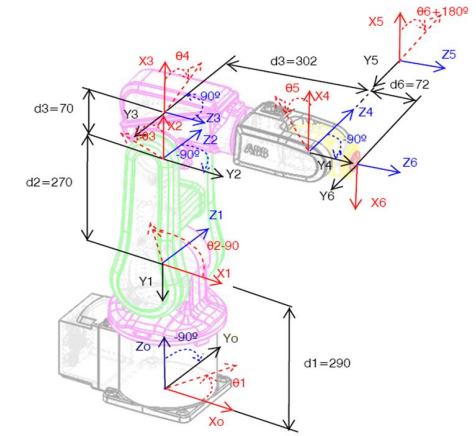
\includegraphics[width=0.75\textwidth]{Immagini/Parametri_DH}
	\caption{Rappresentazione dei parametri di Denavit-Hartenberg} 
	\label{fig:Rappresentazione_DH_Param}
\end{figure}

I parametri nella tabella \ref{tab:DH_Parameters} permettono di andare a rappresentare la matrice di trasformazione generica di un braccio: la matrice~\vref{mat:DH_4MatrixMoltiplication} permette di descrivere la trasformazione che il braccio (\emph{link}) introduce sui due giunti che si trovano alla sua estremità.

Per ricavare invece la matrice di trasformazione omogenea  
$\prescript{i-1}{i}{\textsc{T(q\ped{i})}}$, si vanno ad aggiungere tre terne ausiliarie $\{P\}$,$\{Q\}$ ed $\{R\}$, andando a scrivere le matrici di rotazioni che descrivono ciascuna di essa rispetto a quella precedente (computazione omessa in questa sede).

Andando poi a sfruttare la teoria della composizione di matrici di rotazione  (valida anche per le matrici di trasformazione omogenee viste nella sezione~\vref{equation:MatrixOmogenous}) possiamo scrivere la matrice che descrive la terna $\{i\}$ rispetto alla terna $\{i-1\}$ attraverso la composizione delle quattro matrici di trasformazione relative agli altrettanti sistemi di riferimento: si tratta di andare a moltiplicare in sequenza, una matrice omogenea che descrive una rotazione, due matrici omogenee che rappresentano altrettante traslazioni ed infine un'altra matrice rappresentate rotazione ottenendo il seguente risultato
\begin{equation}
	\footnotesize
	\label{mat:DH_4MatrixMoltiplication}
	\prescript{i-1}{i}{T}	= \prescript{Q}{R}{T} \prescript{R}{i}{T} \prescript{P}{Q}{T} \prescript{i-1}{P}{T}  =
	\begin{bmatrix}
		\begin{array}{ccc|c}
			\begin{matrix}
				\cos \ped{\theta_i}\\
				\sin \ped{\theta_i}\\	
				0
			\end{matrix}
			& 
			\begin{matrix}
				-\sin \ped{\theta_i} \cos \ped{\alpha\ped{i}}\\
				\cos\ped{\theta_i} \cos \ped{\alpha\ped{i}}\\	
				\sin \ped{\alpha\ped{i}}
			\end{matrix}
			&
			\begin{matrix}
				\sin \ped{\theta_i} \sin\ped{\alpha\ped{i}}\\
				-\sin \ped{\alpha\ped{i}}\\	
				\cos \ped{\alpha\ped{i}}
			\end{matrix}
			&
			\begin{matrix}
				a\ped{i} \cos \ped{\theta_i}\\
				a\ped{i} \sin \ped{\theta{i}}\\
				d_i
			\end{matrix}
			\\
			\hline
			0 & 0 & 0 & 1
		\end{array}
	\end{bmatrix}
\end{equation}

Quanto detto finora rappresenta la via risolutiva per risolvere la cinematica diretta del manipolatore in esame: andando ad analizzare ogni singola matrice di trasformazione $i-esima$ possiamo evidenziare ed isolare i seguenti passaggi (con la scritta $s_i$ si indica il valore $\cos \theta_{i}$ e con $s_i$ si rappresenta invece il $\sin\theta_{i}$). 
\begin{equation*}
	\prescript{0}{1}{T}	= A_1 =
	\begin{bmatrix}
		c_1 & 0    &-s_1& 0\\
		s_1 & 0    &c_1 & 0\\
		0   & -1   & 0  & 290\\
		0   & 0    &  0 & 1
	\end{bmatrix}
\end{equation*}\\

\begin{equation*}
	\prescript{1}{2}{T}	= A_2
	\begin{bmatrix}
		c_2 &-s_2 &  0 & 270c_2\\
		s_2 & c_2 &  1 & 270s_2\\
		0   & 0   &  1 & 0\\
		0   & 0   &  0 & 1
	\end{bmatrix}
\end{equation*}\\

\begin{equation*}
	\prescript{2}{3}{T}	= A_3
	\begin{bmatrix}
		c_3 & 0    &-s_3& 70c_3\\
		s_3 & 0    & c_3& 70s_3\\
		0   & -1   & 0  & 0\\
		0   & 0    & 0 & 1
	\end{bmatrix}
\end{equation*}\\

\begin{equation*}
	\prescript{3}{4}{T}	= A_4
	\begin{bmatrix}
		c_4 & 0    &s_4 & 0\\
		s_4 & 0    &-c_4& 0\\
		0   & 1    & 0  & 302\\
		0   & 0    & 0  & 1
	\end{bmatrix}
\end{equation*}

\begin{equation*}
	\prescript{4}{5}{T}	= A_5
	\begin{bmatrix}
		c_5 & 0    &-s_5& 0\\
		s_5 & 0    &c_5 & 0\\
		0   & -1   & 0  & 0\\
		0   & 0    & 0  & 1
	\end{bmatrix}
\end{equation*}

\begin{equation*}
	\prescript{5}{6}{T}	= A_6
	\begin{bmatrix}
		c_6 & -s_6 & 0  & 0\\
		s_6 & c_6  & 0  & 0\\
		0   & 0    & 1  & 72\\
		0   & 0    & 0  & 1
	\end{bmatrix}
\end{equation*}

L'ultimo step per poter giungere così alla risoluzione del problema cinematico diretto per il manipolatore IRB 120 è quello di andare a comporre le informazioni in merito alle roto-traslazioni di ogni sistema di riferimento, partendo dalla base e giungendo fino all'end-effector, ottenendo così posizione e orientamento dello stesso (per non appesantire ulteriormente il discorso, il risultato viene espresso in forma compatta).
\begin{figure}[h]
	\label{fig:Sol_DirectKin}
	\begin{equation*}
		\prescript{0}{6}{T}	= \prescript{0}{1}{T} \prescript{1}{2}{T} \prescript{2}{3}{T} \prescript{3}{4}{T} \prescript{4}{5}{T} \prescript{5}{6}{T}  = A_1A_2A_3A_4A_5A_6
		\begin{bmatrix}
			R_{11} & R_{12} & R_{13} & P_x\\
			R_{21} & R_{22} & R_{23} & P_y\\
			R_{31} & R_{32} & R_{33} & P_z\\
			0    & 0    & 0    & 1
		\end{bmatrix}
	\end{equation*}	
	\caption{Soluzione cinematica diretta manipolatore ABB IRB 120}
\end{figure}

\subsection{Cinematica inversa IRB 120}
Come visto nella matrice in figura~\vref{fig:Sol_DirectKin}, il problema cinematico diretto è sempre risolvibile attraverso la valutazione della matrice di trasformazione omogenea  $\prescript{0}{6}{T}$.

Il problema inverso invece, risulta essere più complicato: infatti, in base alla posizione spaziale fornita tramite coordinate $(x,y,z)$, ci possono essere casi in cui vi è un'unica soluzione, altri in cui ve ne possono essere multiple e altri ancora in cui non vi è alcuna possibile soluzione (quando per esempio la coordinata che si chiede di raggiungere si trova fuori dal range di azione del manipolatore stesso).

Non è quindi garantita nè l'esistenza nè l'unicità della soluzione della cinematica inversa e, nel caso ci siano più soluzioni possibili, si cerca di scegliere la migliore, andando a minimizzare i movimenti dei giunti.

Uno dei più intuitivi modi per poter risolvere il problema cinematico inverso, è quello di andare ad eguagliare la matrice di trasformazione dell'end-effector, che ne indica posizione ed orientamento rispetto alla base, con la sua espressione simbolica, ovvero la matrice che assegna un legame matematico a tutta la catena cinematica del manipolatore (figura~\vref{fig:Sol_DirectKin}).
\begin{figure}[h]
	\begin{equation*}
	\label{mat:InputInverseKin}
	\prescript{0}{6}{T}	= 
	\begin{bmatrix}
	n_x & o_x & a_x & P_x\\
	n_y & o_y & a_y & P_y\\
	n_z & o_z & a_z & P_z\\
	0   & 0   & 0   & 1
	\end{bmatrix}
	\end{equation*}	
	\caption{Input problema cinematico inverso}
\end{figure} 

Si ottengono in questo modo 12 equazioni in 6 incognite: le 9 equazioni della componente di rotazione non sono indipendenti, e si ottengono quindi 6 equazioni in 6 incognite (le variabili di giunto). 

Sicuramente questo rappresenta un metodo stabile per giungere alla soluzione del problema cinematico inverso: dovendo andare a lavorare con un manipolatore avente 6 gdl, l'inversione cinematica non è del tutto agevole, soprattutto per la complessità della parte matematica e di calcolo matriciale.
Conviene quindi andare a studiare il sistema in due parti separate: sfruttando il \emph{disaccoppiamento cinematico}, che si basa su un approccio geometrico-matematico, possiamo infatti studiare separatamente i primi tre giunti, che permettono di posizionare il polso in un punto desiderato, dagli ultimi tre, i quali servono per far assumere allo strumento di lavoro un qualsiasi orientamento.
\subsection{Posizione dell'end-effector: definizione variabili di giunto $\theta_1 - \theta_2 - \theta_3$}
Come detto, il primo approccio applicabile è quello di andare a lavorare sulle matrici di trasformazione ($A_i$), uguagliando
\begin{equation*}
		\prescript{0}{6}{T}	= \prescript{0}{1}{T} \prescript{1}{2}{T} \prescript{2}{3}{T} \prescript{3}{4}{T} \prescript{4}{5}{T} \prescript{5}{6}{T}  = A_1A_2A_3A_4A_5A_6 = 		
		\begin{bmatrix}
			n_x & o_x & a_x & P_x\\
			n_y & o_y & a_y & P_y\\
			n_z & o_z & a_z & P_z\\
			0   & 0   & 0   & 1
		\end{bmatrix} 
\end{equation*}

Per trovare le 6 variabili di giunto andremo quindi a pre-moltiplicare la matrice di trasformazione omogenea $\prescript{0}{6}{T}$ per $A_n^{-1}$, partendo con $A_1^{-1}$:
\begin{figure}[h]
	\label{fig:Metodo_matematico_InvKin}
	\centering
	\begin{equation*}
		A_1^{-1}\times 
		\begin{bmatrix}
			n_x & o_x & a_x & P_x\\
			n_y & o_y & a_y & P_y\\
			n_z & o_z & a_z & P_z\\
			0   & 0   & 0   & 1
		\end{bmatrix}
		=A_2A_3A_4A_5A_6
	\end{equation*}	
\end{figure}


Ci si rende conto da subito come l'onere computazionale a livello matematico sia molto importante; il risultato sopra è ottenibile anche tramite le coordinate spaziali dell'end-effector, che permettono di andare ad imporre una risoluzione tramite metodo geometrico.

Trovando le coordinate del centro del polso nel sistema di riferimento fisso della base e sfruttando la matrice di trasformazione omogenea che viene fornita come input al problema cinematico inverso, possiamo creare un triangolo immaginare che ci permette di definire le coordinate del polso.
\begin{figure}[h]
	\caption{Coordinate del centro del polso del manipolatore}
	\label{fig:Coord_Polso}
	\centering
	\begin{equation*}
		\begin{cases}
			x_P= P_x - 72a_x\\
			y_P= P_y - 72a_y\\
			z_P= P_z - 72a_z		
		\end{cases}
	\end{equation*}
\end{figure}

Possiamo così andare a seguire un semplice ragionamento sul triangolo rettangolo individuato dalle coordinate $x_p$ e $y_p$ del polso, nel quale, l'angolo compreso tra l'ipotenusa e il cateto individuato dalla direzione x è proprio l'angolo $\theta_1$che cerchiamo (vedi figura~\vref{fig:Rappresentazione_DH_Param}), ovvero
\begin{equation*}
	\centering
	\theta_{1,1} = \tan^{-1} \bigl(\frac{y_P}{x_P})
\end{equation*}
\begin{equation*}
	\centering
	\theta_{1,2} = \theta_1+\ang{180}
\end{equation*}
La stesso risultato riportato nelle equazioni soprastanti è ottenibile servendosi della funzione \emph{atan2} (sottosezione~\vref{subsub:Function_atan2}), ottenendo come risultato
\begin{equation*}
	\centering
	\theta_{1,1} = \atantwo(y_P,x_P)
\end{equation*}
\begin{equation*}
	\centering
	\theta_{1,2} = \atantwo(-y_P,-x_P)
\end{equation*}

Secondo un ragionamento molto simile, possiamo andare a calcolare $\theta_2$: si vede come, effettuando un ragionamento sui triangoli evidenziati in figura~\vref{fig:CalcoloTheta2}, possiamo evidenziare come l'angolo $\beta$ sia pari all'angolo $(\theta_2-\ang{90})-\gamma$.
\begin{figure}
	\centering
	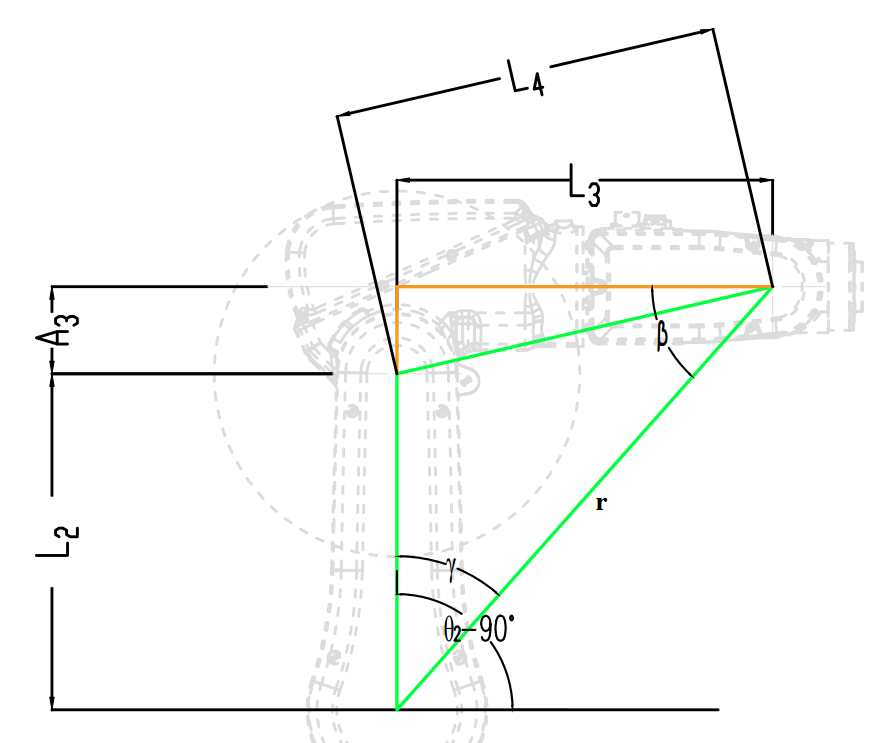
\includegraphics[width=0.75\textwidth]{Immagini/Theta_2_2}
	\caption{Triangoli di supporto per il calcolo del angolo $\theta_2$} 
	\label{fig:CalcoloTheta2}
\end{figure}

La lunghezza di $r$ dipende però ovviamente anche da altri angoli (quali $\theta_3$ per esempio): per procedere con il suo calcolo andiamo a ricavare le coordinate del polso (figura~\vref{fig:Coord_Polso}) espresse però nel sistema di riferimento 1 la cui origine si trova nel vertice dove è presente l'angolo $\theta_2-\ang{90}$, cioè dove si "ancora" il primo braccio del manipolatore. 

Quest'origine la possiamo definire andando a trovare la matrice di Denavit-Hartenberg relativa al sistema di riferimento 1 e poi, con una semplice moltiplicazione matriciale, siamo in grado di ottenere le coordinate del polso rispetto al punto prima specificato. 
\newpage
Conoscendo queste coordinate risulta facile calcolare sia il valore dell'angolo $\beta$ sia dell'angolo $\gamma$ (sfruttando il teorema di Carnot). 

Lo script \emph{MATLAB} risultante dai ragionamenti effettuati è il seguente:


\begin{lstlisting}[style=Matlab-editor,caption=Calcolo del parametro di giunto $\theta_2$,captionpos=b,label={Code:theta2}, basicstyle=\footnotesize\ttfamily,frame=trBL]

	%Parametri di Denavit-Hartenberg
	L2=270; %a_2
	L3=302; %d_4
	A3=70; %a_3	
	
	%Calcolo della lunghezza L_4
	L4 = sqrt(A3^2 + L3^2);

	%Matrice di trasformazione omogenea del primo giunto: indica orientamento e posizione del primo sistema di  riferimento rispetto alla base
	T01=Calcolo_DH_Matrix(robot, q, 1);	
	
	%Esprimo le coordinate del centro del polso rispetto alla base, utilizzando il concetto espresso in figura 2.18
	p1 = inv(T01)[Pm; 1];
	
	%Calcolo la distanza r, che dipende quindi dalla posizione del centro del polso e non risulta essere costante
	r = sqrt(p1(1)^2 + p1(2)^2);
	
	%Calcolo gli angoli espressi in figura 2.20, utilizzando i concetti matematici precedentemente esposti
	beta = atan2(-p1(2), p1(1));
	gamma = real(acos((L2^2+r^2-L4^2)/(2*r*L2)));	
	
	%Ho due possibili soluzioni: gomito su e gomito giu'
	q2(1) = pi/2 - beta - gamma;
	q2(2) = pi/2 - beta + gamma;
\end{lstlisting}




Per il calcolo di $\theta_3$ i parametri geometrici, ovvero le lunghezza dei lati dei triangoli presi in considerazione, sono sempre quelli presentati nel codice~\vref{Code:theta2}, cambia solamente il calcolo dell'angolo, come è ovvio che sia, il quale può essere così sviluppato:

\begin{lstlisting}[style=Matlab-editor,caption=Calcolo del parametro di giunto $\theta_3$,captionpos=b,label={Code:theta3}, basicstyle=\footnotesize\ttfamily,frame=trBL]

	%Calcolo degli angoli caratterizzanti
	phi=acos((A3^2+L4^2-L3^2)/(2*A3*L4));
	eta = real(acos((L2^2 + L4^2 - r^2)/(2*L2*L4)));
	
	%Due possibili soluzioni: gomito su e gomito giu
	q3(1) = pi - phi- eta; 
	q3(2) = pi - phi + eta; 
\end{lstlisting}



\begin{figure}[h]
	\centering
	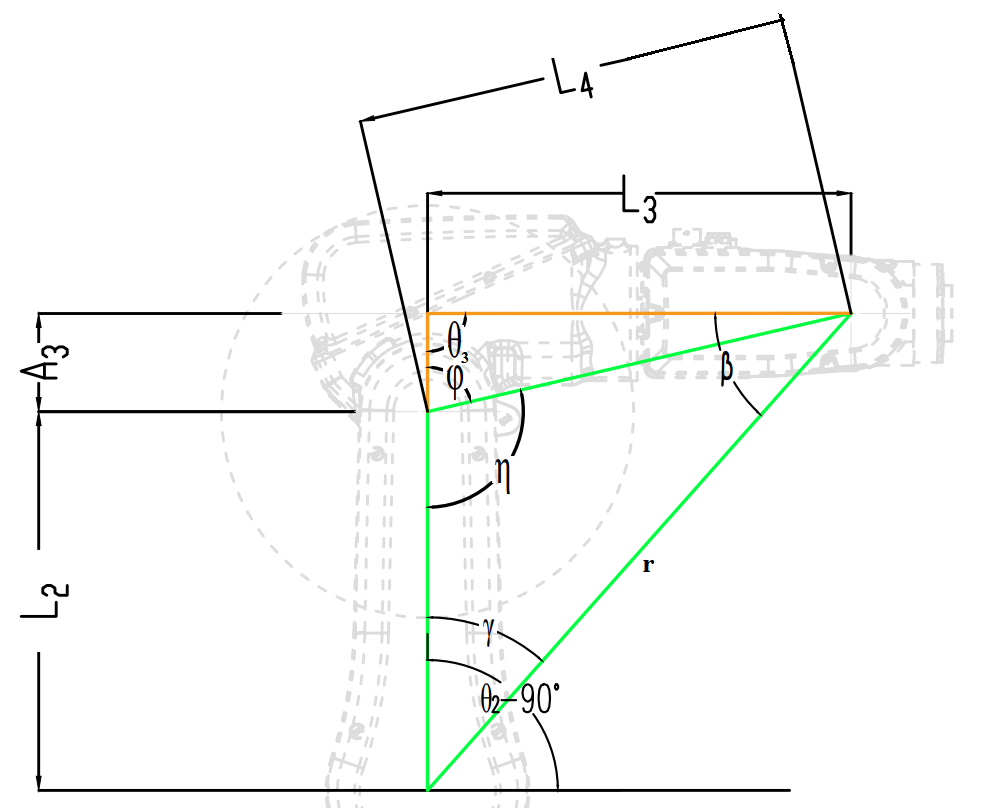
\includegraphics[width=0.75\textwidth]{Immagini/Theta_3}
	\caption{Triangoli di supporto per il calcolo del angolo $\theta_3$} 
	\label{fig:CalcoloTheta3}
\end{figure}



\subsection{Orientamento dell'end-effector: definizione variabili di giunto $\theta_4 - \theta_5 - \theta_6$}
Una volta calcolati i valori di $\theta_1 - \theta_2 - \theta_3$, la posizione del centro del polso risulta essere fissata: possiamo quindi calcolare la matrice di trasformazione omogenea che descrive la catena cinematica degli ultimi tre giunti.

\begin{lstlisting}[style=Matlab-editor,caption=Matrice  di trasformazione omogenea dei primi tre giunti,captionpos=b,label={Code:MatTrasf}, basicstyle=\footnotesize\ttfamily,frame=trBL]

	%Calcolo della posizione e dell'orientamento del terzo sistema di riferimento utilizzando gli angoli q (theta_1,theta_2,theta_3) prima calcolati
	T01=DH_Compute(robot, q, 1);
	T12=DH_Compute(robot, q, 2);
	T23=DH_Compute(robot, q, 3);
	T03=T01*T12*T23;
	
	%Vado ad estrarre le informazioni in merito alla rotazione del sistema di riferimento, come rappresentato in figura 2.10.
    x3=T03(1:3,1);
	y3=T03(1:3,2);
	z3=T03(1:3,3);
\end{lstlisting}
Questo listato fornisce la posizione del polso: quello che andiamo ora a fissare, definendo i tre angoli $\theta_4 - \theta_5 - \theta_6$ è l'orientamento del polso stesso, che può essere definito in termini di angoli di Eulero, ovvero di rollio-beccheggio-imbardata (\emph{Raw-Pitch-Yaw}). Come fatto precedentemente per individuare la posizione, anche qui abbiamo due vie di risoluzione: potremmo andare a risolvere il problema inverso tramite una via algebrica, la quale si basa sugli angoli individuati precedentemente ($\theta_1 - \theta_2 - \theta_3$) partendo dalla formula in figura~\vref{fig:AlgebricSolution}.
\begin{figure}
	\centering
	\caption{Step iniziale per il calcolo algebrico dell'orientamento del polso}
	\label{fig:AlgebricSolution}
	\begin{equation*}
		A_4A_5A_6 = (A_1A_2A_3)^{-1}		
		\begin{bmatrix}
		n_x & o_x & a_x & P_x\\
		n_y & o_y & a_y & P_y\\
		n_z & o_z & a_z & P_z\\
		0   & 0   & 0   & 1
		\end{bmatrix} 
	\end{equation*}
\end{figure}

Un altro possibile approccio, decisamente meno oneroso a livello computazionale, è rappresentato ancora una volta da quello geometrico: andando a lavorare sull'orientamento dei vari sistemi di riferimento rappresentati in figura~\vref{fig:CalcoloOrientamentoWrist} siamo in grado di recuperare i valori di $\theta_4 - \theta_5 -\theta_6$. 
\begin{figure}
	\centering
	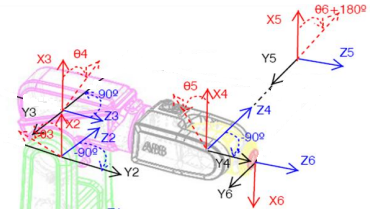
\includegraphics[width=0.75\textwidth]{Immagini/SistemiDiRiferimento_OrientamentoWrist}
	\caption{Sistemi di riferimento dei giunti utilizzati per trovare l'orientamento del polso} 
	\label{fig:CalcoloOrientamentoWrist}
\end{figure}

L'approccio che possiamo seguire per poter trovare l'angolo $\theta_4$ è quello di andare a studiare l'orientamento dell'asse $z_3$ e $z_6$, il quale è fornito in ingresso al problema cinematico inverso: valutando la posizione reciproca dei due assi sopracitati, possiamo andare a definire due casistiche di valori per $\theta_4$. In un caso esso è nullo, nell'altro può essere trovato andando sostanzialmente a costruire un triangolo rettangolo intorno a $\theta_4$, i cui lati possono essere considerati come gli assi $x_3$, $y_3$ e $z_3$.

Come si può notare nella figura~\vref{fig:CalcoloOrientamentoWrist}, $\theta_4$ è proprio l'angolo che si crea con $x_3$ e la trasposizione di $z_4$ sul giunto numero 3: operando un prodotto scalare, siamo in grado di trovare la proiezione di $z_4$ dapprima lungo $x_3$ e successivamente lungo $y_3$, grazie al significato geometrico proprio del prodotto scalare tra vettori.

Questi passaggi permettono di ottenere nient'altro che il valore del $cos$ e del $sen$ dell'angolo $\theta_4$, legati tra loro dalla funzione $atan$, come si può vedere nel codice~\vref{Code:theta4}.

\begin{lstlisting}[style=Matlab-editor,caption=Calcolo di $\theta_4$,captionpos=b,label={Code:theta4}, basicstyle=\footnotesize\ttfamily,frame=trBL]
	%Vado a calcolare la matrice di trasformazione omogenea del terzo giunto sfruttando le proprieta' delle matrici di trasformazione
	T01=DH_Compute(robot, q, 1);
	T12=DH_Compute(robot, q, 2);
	T23=DH_Compute(robot, q, 3);
	T03=T01*T12*T23;
	
	%Orientamento dei tre assi del sistema di riferimento del terzo giunto
	x3=T03(1:3,1);
	y3=T03(1:3,2);
	z3=T03(1:3,3);

	%Asse z_6 che corrisponde al vettore a nella matrice di trasformazione in input al problema cinematico inverso
	a=T(1:3,3);
	
	%Prodotto vettoriale: il risultato e' un vettore ortogonale al piano individuato da z_3 e z_6
	z4=cross(z3, a);   
	
	%Il modulo rappresenta l'area compresa tra i due assi: se e' circa nulla, vuol dire che i due assi sono paralleli, per le proprieta' del prodotto vettoriale
	if norm(z4) <= 0.000001
		q(4)=0;
	else
		%Vado a compormi un triangolo rettangolo, in base a quello che e' l'orientamento della sesta terna
		cq4=wrist*dot(z4, -y3);
		sq4=wrist*dot(z4, x3);
		q(4)=atan2(	sq4, cq4);
	end
\end{lstlisting}
\newpage
Anche per il calcolo di $\theta_5$ possiamo andare ad operare lo stesso ragionamento fatto per trovare $\theta_4$: in questo caso troveremo la proiezione dell'asse $z_5$, il quale fa riferimento al giunto 5 in esame, sugli assi del giunto precedente, ovvero su  $x_4$ e $y_4$.
\begin{lstlisting}[style=Matlab-editor,caption=Calcolo di $\theta_5$,captionpos=b,label={Code:theta5}, basicstyle=\footnotesize\ttfamily,frame=trBL]
	%Progressiva ricostruzione dell'orientamento e posizione della catena cinematica del manipolatore
	T34=DH_Compute(robot, q, 4);
	T04=T03*T34;
	x4=T04(1:3, 1);
	y4=T04(1:3, 2);
	
	%L'asse z_5 ha la stessa direzione di z_6
	z5=T(1:3, 3); 
	
	%Vado a lavorare sul triangolo rettangolo formato dagli assi	
	cq5=dot(z5, y4);
	sq5=dot(z5, -x4);
	q(5)=atan2(sq5, cq5);
\end{lstlisting}
Ripetiamo infine lo stesso concetto geometrico presentato per il calcolo di $\theta_4$ e $\theta_5$, anche per andare a trovare il valore di $\theta_6$.
\begin{lstlisting}[style=Matlab-editor,caption=Calcolo di $\theta_6$,captionpos=b,label={Code:theta6}, basicstyle=\footnotesize\ttfamily,frame=trBL]
	x6=T(1:3, 1);
	
	T45=DH_Compute(robot, q, 5);
	T05=T04*T45;
	x5=T05(1:3, 1);
	y5=T05(1:3, 2);
	
	cq6=dot(x6, -x5);
	sq6=dot(x6, -y5);
	q(6)=atan2(sq6, cq6);

\end{lstlisting}

\subsubsection{Quaternioni}
Nello studio della cinematica inversa si è analizzato come le variabili note a priori, per poter giungere alla soluzione del problema stesso, sono la posizione e l'orientamento dell'end-effector rispetto alla base del manipolatore stesso. 

Come visto nel paragrafo~\vref{subsub:Rot_elementari} si è in grado di esprimere la rotazione di una terna mobile rispetto ad una fissa traimite una matrice detta \emph{matrice di rotazione}: un modo però più conciso per poter esprimere l'informazione in merito alla rotazione è rappresentato dall'utilizzo dei quaternioni. 
Essi rappresentano delle entità in forma complessa che, data una matrice di rotazione in questa forma
\begin{equation}
	\centering
	\begin{bmatrix}
		x_1&y_1&z_1\\
		x_2&y_2&z_2\\	
		x_3&y_3&z_3
	\end{bmatrix}
\end{equation}
possono essere ottenuti come:
\begin{table}[h]
	\label{tab:Quaternion}
	\centering
	\begin{tabular}{cc}
			\midrule
			$q_1=\frac{\sqrt{x_1+y_2+z_3+1}}{2}$ & \\ 
			$q_2=\frac{\sqrt{x_1-y_2-z_3+1}}{2}$ & $sign q_2 = sign(y_3-z_2)$ \\
			$q_3=\frac{\sqrt{y_2-x_1-z_3+1}}{2}$ & $sign q_3 = sign(z_1-x_3)$ \\
			$q_4=\frac{\sqrt{z_3-x_1-Y_2+1}}{2}$ & $sign q_4 = sign(x_2-y_1)$ \\
			\bottomrule  
	\end{tabular}
\end{table}

\subsubsection{La funzione atan2}
\label{subsub:Function_atan2}
Sempre nella risoluzione della cinematica inversa, per andare a calcolare i 6 parametri di giunto, si vanno ad utilizzare concetti geometrici-matematici, richiamando soprattutto la geometria riguardante i triangoli rettangoli. 
Nello specifico, è importante saper gestire quello che è il corretto segno da assegnare agli angoli calcolati, e questo viene ad essere fatto tramite la funzione $\atantwo$ la quale segue il comportamento presentato in figura~\vref{fig:atan2}.

\begin{figure}[h]
	\centering
	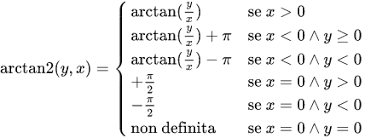
\includegraphics[width=0.65\textwidth]{Immagini/atan2}
	\caption{Caratteristiche della funzione $\atantwo$}
	%[Immagine presa dal sito https://it.wikipedia.org/wiki/Arcotangente2 in data 18/03/18]
	\label{fig:atan2}
\end{figure}
%======================================================================